\documentclass[12pt, a4paper]{article}
\usepackage{mathtext}
\usepackage[utf8x]{inputenc}
\usepackage[russian]{babel}
\usepackage{amsmath}
\usepackage{amsfonts}
\usepackage{amssymb}
\usepackage{latexsym}
\usepackage[left=2cm,right=1.25cm,
    top=1.5cm,bottom=1.5cm,bindingoffset=0cm]{geometry}
\usepackage{graphicx}
\usepackage[font=small,labelfont=bf]{caption}

\begin{document}
% НАЧАЛО ТИТУЛЬНОГО ЛИСТА
\begin{center}
\hfill \break
\footnotesize{ФЕДЕРАЛЬНОЕ ГОСУДАРСТВЕННОЕ АВТОНОМНОЕ ОБРАЗОВАТЕЛЬНОЕ УЧРЕЖДЕНИЕ}\\ 
\footnotesize{ВЫСШЕГО ОБРАЗОВАНИЯ}\\
\small{\textbf{«НАЦИОНАЛЬНЫЙ ИССЛЕДОВАТЕЛЬСКИЙ УНИВЕРСИТЕТ \\ «ВЫСШАЯ ШКОЛА ЭКОНОМИКИ»}}\\
\hfill \break
\normalsize{Факультет экономических наук}\\
\normalsize{Образовательная программа «Экономика»,}\\
\normalsize{по направлению 38.03.01 «Экономика»}\\
 \hfill \break
\hfill\break
\hfill\break
\hfill \break
\hfill \break
\hfill \break
 \hfill \break
 \hfill \break
 \hfill \break
 \hfill \break
\normalsize{Коломоец Эвелина Вячеславовна, Нагорская Мария Александровна}\\
\large{\textbf{АНАЛИЗ ФАКТОРОВ, ВЛИЯЮЩИХ НА СРЕДНЮЮ ПРОДОЛЖИТЕЛЬНОСТЬ РАБОЧЕЙ НЕДЕЛИ}}\\
\hfill \break
\hfill \break
\hfill \break
\normalsize{Проект по предмету «Эконометрика-2»}\\
\hfill \break
\hfill \break
\end{center}



\normalsize{ 
\hfill\break\hfill\break\hfill\break\hfill\break\hfill\break\hfill\break\hfill\break\hfill\break\hfill\break\hfill\break\hfill\break\hfill\break\hfill\break\hfill\break\hfill\break
\hfill \break
\hfill \break
\begin{center} Москва 2024 \end{center}
\thispagestyle{empty} % выключаем отображение номера для этой страницы
 
\newpage
\section{Введение}

Найти баланс между работой и отдыхом – то, к чему стремится каждый человек, достигая определенного возраста. Наступил тот самый момент, когда авторы данной работы также задумались об этом вопросе. Исследования показывают, что для поддержания качества жизни на высоком уровне необходимо следить за количеством часов в рабочей неделе. Переработки могут привести к ряду негативных последствий, например, к ухудшению здоровья работника, риску профессионального выгорания и увеличению несчастных случаев на работе (Stewart et al., 2019).

Интересен тот факт, что средняя продолжительность рабочей недели может значительно различаться в бедных и богатых странах. Для стран с низким уровнем дохода и/или развивающихся стран характерна более продолжительная рабочая неделя, нежели для развитых стран с высоким уровнем жизни и большим количеством социальных гарантий (Fuchs-Schündeln, 2019). Что касается России, то начиная с 90-х годов продолжительность рабочего времени в производственной сфере планомерно увеличивается, а в непроизводственной — уменьшается (Зайкова И., 2020).

Согласно (Newton et al. 1979) на среднюю продолжительность рабочей недели сильно влияют семейные обязательства, которые могут подавлять желание работников выбирать больше свободного времени в обмен на высокий доход. Кроме того, в статьях отмечают, что на времени, которое человек уделяет работе, сказывается занимаемая им позиция. Так, например, более 40\% менеджеров работают 45 часов или больше, в то время как только 5\% офисных работников и 17\% промышленных работников работают такое же количество часов (Boisard et al., 2003).

Таким образом, у исследователей существуют разные мнения, почему люди работают больше или меньше часов в неделю. Для понимания истинных мотивов и обстоятельств, побуждающих людей работать сверх установленного времени, актуально будет систематизировать факторы, влияющие на продолжительность рабочей недели в России в настоящее время.

\subsection{Основные гипотезы}

Зачастую специфика отрасли влияет на количество затраченных на выполнение задач часов. Согласно исследованию (Зайкова И., 2020), люди в производственной сфере тратят на работу все больше и больше времени в неделю. В связи с этим сформулирована следующая гипотеза:

1.  Занятость в производственной отрасли сильнее влияют на продолжительность рабочей недели, чем в непроизводственной (то есть коэффициенты при дамми-переменных, отражающих производственные отрасли, будут значимыми)

В качестве производственных отраслей были определены: деревообрабатывающая промышленность, лесное хозяйство, химическая промышленность, энергетическая промышленность, строительство, другая отрасль тяжелой промышленности, нефтегазовая промышленность, военно-промышленный комплекс, гражданское машиностроение, легкая, пищевая промышленность.

По мнению (Boisard et al., 2003) на продолжительность рабочей недели влияет должность, которую занимает человек. Как правило, чем выше должность, тем больше подчиненных имеет работник. И в данном контексте могут быть два варианта развития событий: либо человек умеет делегировать задачи подчиненным и поэтому сильно не перерабатывает, либо большая ответственность побуждает его тратить больше часов на выполнение рабочих задач. На основе этого предполагаем следующую гипотезу:

2.  Чем больше подчиненных имеет работник, тем больше часов будет длиться его рабочая неделя (то есть коэффициент при переменной, показывающей количество подчиненных у человека, будет положительным)

Наконец, будучи студентами НИУ ВШЭ, авторы работы считают важным наличие высшего образования для дальнейшей карьеры. Люди, у которых нет достаточной квалификации, в основном задействованы в той сфере, где не требуется высокая умственная активность, и часто эти сферы связаны с физической работой, которая может занимать больше времени. С надеждами выдвигается третья гипотеза:

3.  Чем ниже уровень образования, тем больше средняя продолжительность рабочей недели (так как мы считаем образование порядковой переменной (подробнее об этом дальше в работе), коэффициент при ней будет отрицательным)

\section{Данные}
Для исследования были выбраны данные индивидуального уровня 31 волны РМЭЗ НИУ ВШЭ (т.е. ответы респондентов представлены по состоянию на 2022 год). Модель выборки этой базы данных — «повторяющаяся выборка» с «разделяющейся панелью», домохозяйства и индивиды выбирались с использованием метода многоступенчатого территориального вероятностного выбора: из 2029 объединённых районов, которые затем были сгруппированы в 38 страт на основании географических факторов, этнической составляющей и уровня урбанизации. В выборке отсутствуют отдалённые и малонаселённые районы, а так же Чеченская Республика (как горячая точка).

\subsection{Переменные}
В изначальном датасете представлены ответы на 741 вопрос от 17 343 индивидов, из них были отобраны 16 переменных:

\textbf{Описание работы и должности}

-   Средняя продолжительность рабочей недели

-   Отрасль работы 

-   Среднемесячная зарплата (в рублях)

-   Является ли производство вредным/опасным

-   Использовался ли за последние 12 месяцев интернет для работы

-   Наличие подчиненных

-   Количество подчиненных

\textbf{Описание респондента}

-   Пол респондента

-   Возраст респондента (в годах)

-   Образование респондента

-   Трудовой стаж респондента (в годах)

\textbf{Описание места работы}

-   Является ли место работы предприятием

-   Является ли занятость официальной

-   Сколько человек работает на предприятии

-   Является ли государство владельцем / совладельцем предприятия

-   Является ли респондент владельцем / совладельцем предприятия

\subsection{Эндогенность в данных}

Отметим, что продолжительность рабочей недели, зарплата, количество людей в компании в целом и в подчинении (как, впрочем, и другие ответы) записаны со слов респондентов, то есть возможна ошибка измерения: люди склонны округлять числа до некоторого «круглого», например, вместо зарплаты 24 981 рубль сказать 25 000. По мнению авторов, подобные округления, хотя и являются источником эндогенности, не должны значительно влиять на причины переработок и недоработок, а потому будут проигнорированы. 

Однако, из-за эндогенности ощутимое влияние на параметры модели может оказать пропуск ненаблюдаемой переменной «мотивация работать»: логичным кажется предположение, что при нейтральном или незаинтересованном отношении к работе человек будет работать не дольше, чем ему положено, а если же отношение будет негативным — то даже меньше указанных в договоре часов. В таком случае, есть смысл попытаться оценить эту переменную. Предполагается, что понятие «мотивация работать» можно разбить на несколько случаев:

1.  Мотивация как страх потерять работу

    -   Наличие детей

    -   Насколько респондента беспокоит то, что он(а) может потерять работу

2.  Мотивация повышения / сохранения уровня жизни

    -   Удовлетворенность респондента своим материальным положением в настоящее время

    -   Представьте себе лестницу из 9 ступеней, где на нижней, первой ступени, стоят нищие, а на высшей, девятой - богатые. На какой из девяти ступеней респондент считает, что находится

    -   Насколько респондента беспокоит то, что он(а) не сможет обеспечивать себя самым необходимым в ближайшие 12 месяцев

    -   Как респондент думает, через 12 месяцев он(а) и семья будет жить лучше или хуже, чем сегодня?

3.  Отсутствие мотивации

    -   Задерживает ли предприятие зарплату

    -   Сколько денег задерживает (в рублях)

    -   Сколько месяцев задерживает

    -   Хочет ли респондент найти (другую) работу

\subsection{Обработка данных}
В исходном датасете немало пропусков, которые потребовали обработки: были обработаны пропуски, которые можно заполнить по смыслу (например, если респондент ответил, что подчиненных нет, то в вопросе про их количество был проставлен 0) и удалены наблюдения, где пропущена зависимая переменная, а также те, где респондент хотя бы единожды дал неинформативный ответ (например, "Затрудняюсь ответить", "Отказ от ответа" и т.п.). В результате был получен датасет из 3 156 наблюдений. После этого было обнаружено, что переменная "Является ли место работы предприятием" потеряла смысл: она стала принимать единственное значение, а потому была удалена. 

Категориальные переменные, кроме уровня образования, будут преобразованы в дамми-переменные. Уровень образования -- это упорядоченное множество, поэтому считаем целесообразным оставить изначальные значения (чем больше число, тем выше уровень образования). 

\subsection{Предварительный анализ данных}
В данных присутствует дисбаланс, что заметно по описательным статистикам численных переменных: у нескольких из них минимальное значение совпадает с медианным. 
\begin{table}[h] 
\centering 
\caption{Описательные статистики зависимой и объясняющих переменных} 
\label{tab:descriptive_stats} 
\begin{tabular}{@{}p{8cm}ccccc@{}} \hline 
\hline \\[-1.8ex] 
  & Min & Median & Mean & St.Dev. & Max \\
\hline \\[-1.8ex] 
Средняя продолжительность раб.недели (часов)& 4 & 40 & 42.1 & 9.58 & 120 \\
Зарплата & 0 & 31 000 & 37 670 & 24 839.25 & 313 000 \\
Возраст (лет) & 18 & 41 & 42.31 & 11.29 & 83 \\
Стаж (лет) & 0 & 18 & 19.17 & 11.63 & 62 \\
Число подчиненных & 0 & 0 & 3.583 & 55.22 & 3 000 \\
Число человек на предприятии & 1 & 50 & 497.4 & 2 203.65 & 35 000 \\
Сумма, невыплаченная предприятием & 0 & 0 & 141.3 & 2 465.67 & 80 000 \\
Время, за которое не выплачена сумма & 0 & 0 & 0.008 & 0.14 & 6 \\
\hline \\[-1.8ex] 
\end{tabular}
\end{table} 

Также сложно не заметить наличие гетероскедастичности – стандартные ошибки существенно отличаются, в том числе в относительных значениях с учетом отличий в размерности (зарплата измеряется в тысячах, а возраст нет): есть переменные, для которых стандартные ошибки существенно больше среднего, равно как и наоборот. 


\begin{center}
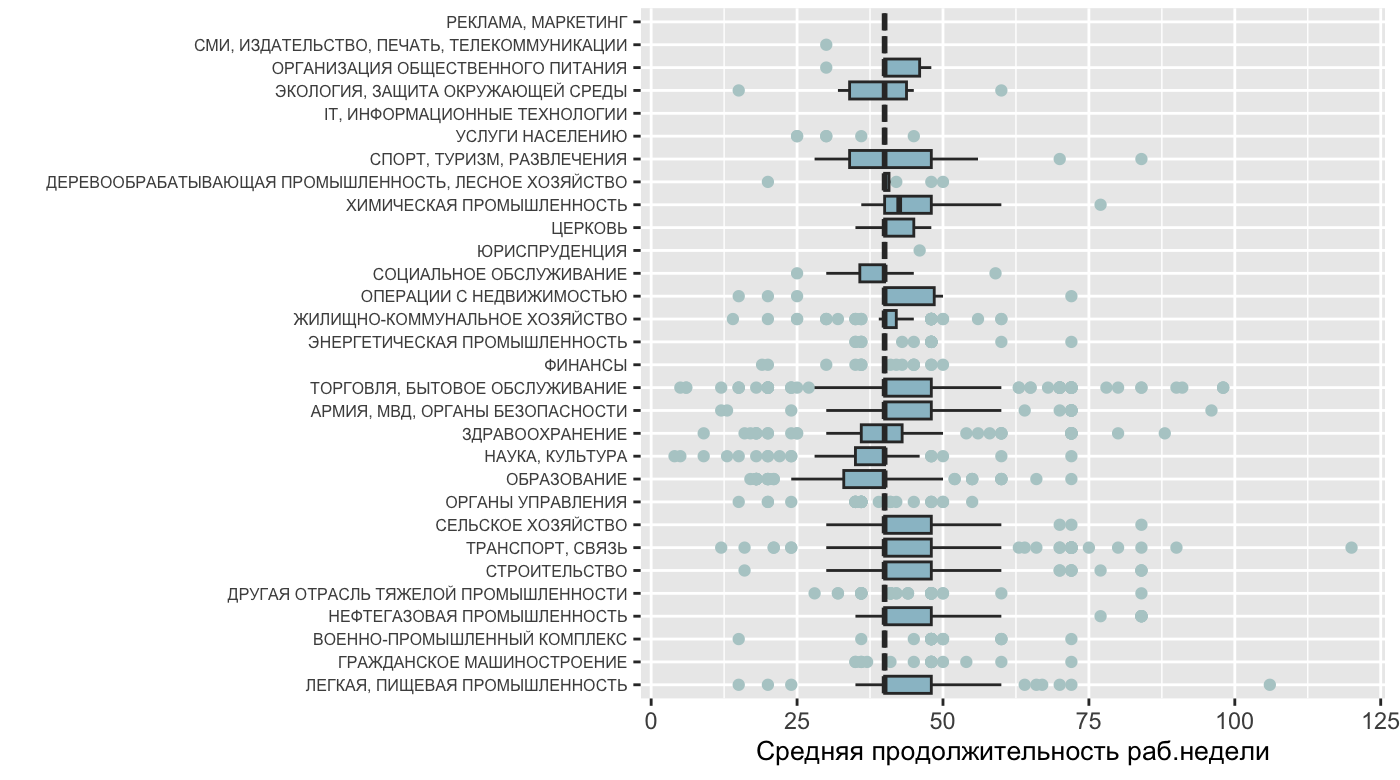
\includegraphics[width=0.6\textwidth]{structure}
\captionof{figure}{Распределение средней продолжительности рабочей недели по отраслям}
\end{center}

Видим, что во многих производственных сферах присутствуют выбросы и продолжительность рабочей недели превышает 40 часов. Для некоторых непроизводственных отраслей, например, образования, науки и культуры не характерны переработки, что достаточно логично, ведь у учителей и преподавателей есть обозначенный график, не всегда охватывающий ровно 40 часов. Однако есть и те непроизводственные отрасли, где рабочая неделя не такая короткая, поэтому проверка гипотезы, обозначенной ранее, актуальна.

\begin{center}
	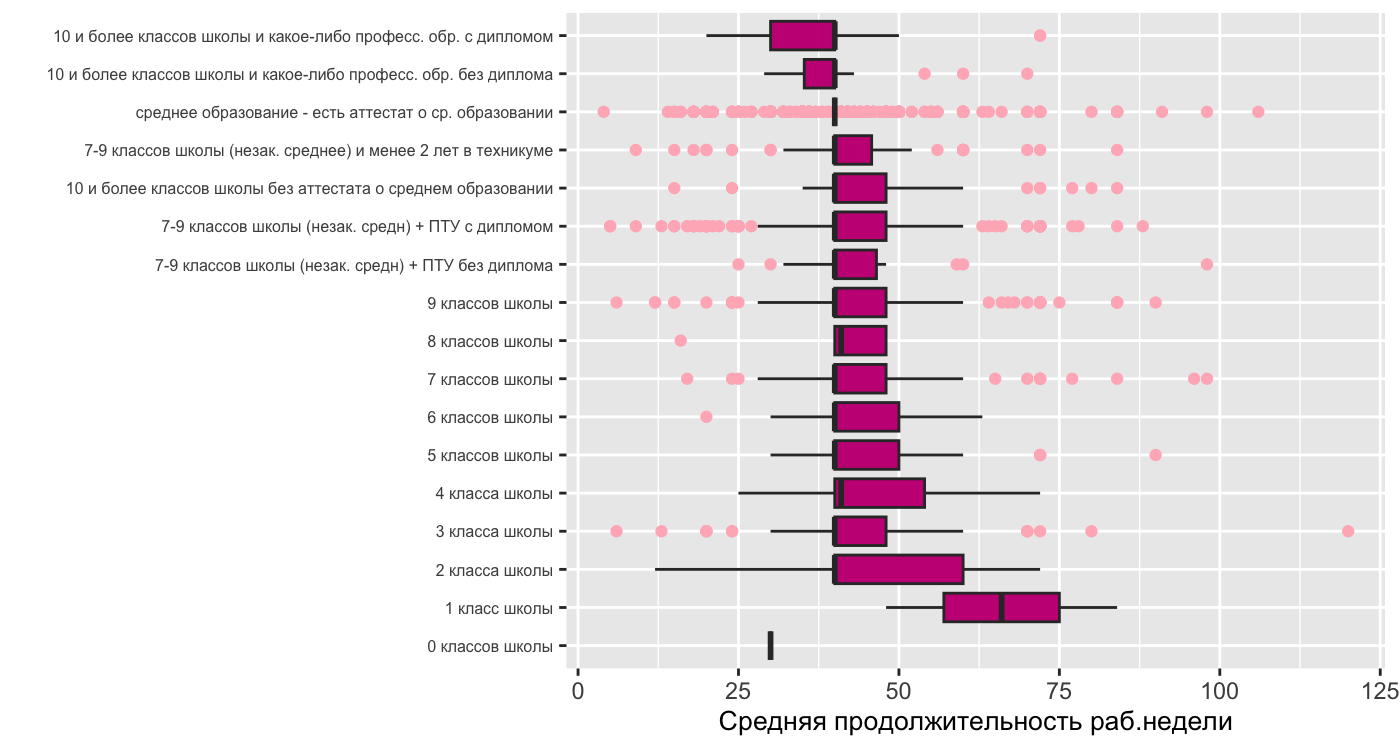
\includegraphics[width=0.6\textwidth]{educ}
	\captionof{figure}{Распределение средней продолжительности рабочей недели в зависимости от уровня образования}
\end{center}

Вызывают интерес индивиды, имеющие образование меньше 9-и классов, так как по закону каждый человек должен получить основное общее образование. Видимо, государство не зря заботится о гражданах, ведь люди, не окончившие 9 классов, работают сильно больше, чем те, у кого более высокий уровень образования. И видно также менее продолжительную рабочую неделю у людей с дипломом, что при визуальном анализе данных подтверждает нашу гипотезу.

\begin{center}
	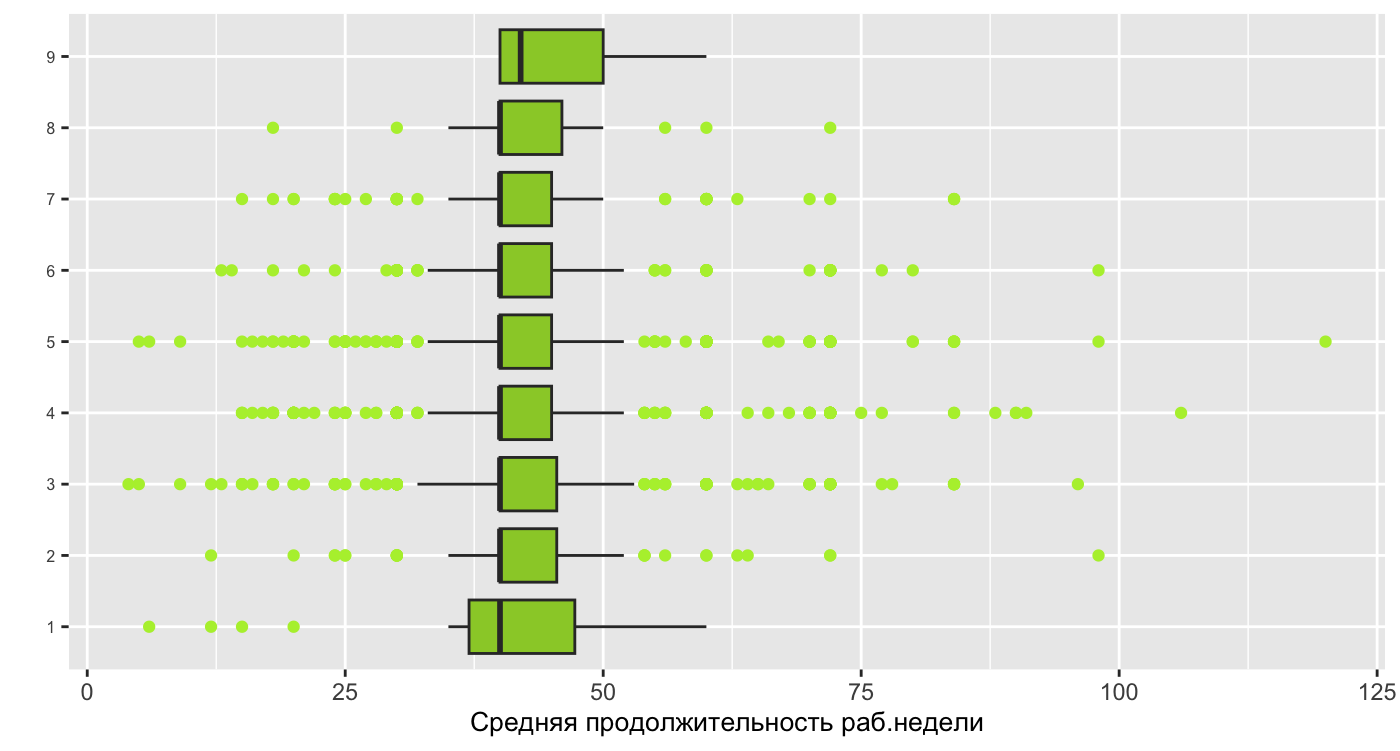
\includegraphics[width=0.6\textwidth]{rich}
	\captionof{figure}{Распределение средней продолжительности рабочей недели в зависимости от того, на какой ступени богатства респондент считает, что находится (1 - беднейший, 9 - богатейший)}
\end{center}
Существует мнение, что богатые люди должны работать больше часов в неделю, в силу больших затрат ресурсов и большей ответственности. Рис. 3 показывает, что зачастую это действительно так. Однако также можно заметить, что и наиболее бедные люди могут работать больше, чем остальные. Микроэкономическая теория о backward-bending кривой  предложения труда тоже мало похожа на правду на этих данных: похожая зависимость будет наблюдаться, если строить кривую через аномальные точки с повышенной продолжительностью рабочей недели, но причины предпочесть эти точки противоположным (с продолжительностью менее 40 часов) отсутствуют.

\section{Модель}
Поскольку в работе используются замещающие, а не инструментальные переменные, модели будут построены стандартными способами: при помощи МНК и при помощи метода максимального правдоподобия, исходя из предположения о нормальности распределения. Обращаясь к результатам предварительного анализа данных, вероятнее всего, потребуется использование робастных ошибок для борьбы с гетероскедастичностью. 

\begin{thebibliography}{9} 

\bibitem{stewart} Stewart J., Frazis H. The importance and challenges of measuring work hours, the IZA World of Labor, 2019
\bibitem{fuchs} Nicola Fuchs-Schündeln Hours Worked Across the World: Facts and Driving Forces, National Institute Economic Review , Volume 247 , February 2019 , pp. R3 - R9
\bibitem{boisard} Boisard P., Cartron D., Valeyre A. Time and work: duration of work, European Foundation for the Improvement of Living and Working Conditions, 2003
\bibitem{zaikova} Зайкова И. Динамика продолжительности рабочего времени в Российской Федерации, «Инновации и инвестиции». № 6. 2020
\bibitem{newton} Newton K., Leckie N. Determinants of Weekly Work Hours in Canada, RELATIONS INDUSTRIELLES, VOL. 34. NO 2 (1979)

\end{thebibliography}


\end{document}
